\documentclass[oneside, 12pt]{article}
\usepackage{tgtermes}
%\renewcommand{\familydefault}{\sfdefault}
\usepackage[english]{babel}
\usepackage{graphicx} % Required for inserting images}
\usepackage{adjustbox} 
\usepackage{amsmath}   % For math symbols
\usepackage{amssymb}
\usepackage{amsthm}
\usepackage[most]{tcolorbox}
\usepackage{lipsum}
\usepackage{tabularx}
\usepackage{array}
\usepackage[most]{tcolorbox} % tcolorbox package for colored, breakable boxes
\usepackage[dvipsnames]{xcolor}
\usepackage{wrapfig}
\usepackage{enumitem}
\usepackage{bbm}
\usepackage{tikz}
\tikzset{every picture/.style={line width=0.75pt}} %set default line width to 0.75pt    g
\usetikzlibrary{shapes.geometric, positioning, arrows.meta} % Ensure proper libraries are loaded
\usetikzlibrary{arrows.meta, decorations.pathreplacing, positioning}
\usepackage{pst-node}
\usepackage{fancyhdr}
\usepackage{pgfplots}
\usepackage{subcaption}
\usepackage{booktabs}
\usepackage{actuarialsymbol}
\pgfplotsset{compat=1.18}
\usetikzlibrary{decorations.pathreplacing}
\usepgfplotslibrary{fillbetween}
\usepackage{forest}
\immediate\write18{which pygmentize > pygmentize-path.txt}
\immediate\write18{Rscript ExamDataset.R}
\usepackage{minted}
\tcbuselibrary{listingsutf8}
\usepackage{etoolbox} % for patching minted
\usepackage[
    letterpaper,
    top=0.9in,
    bottom=0.9in,
    left=0.9in,
    right=0.9in
]{geometry}
\usepackage{listofitems} % for \readlist to create arrays
\usepackage[outline]{contour} % glow around text
\contourlength{1.4pt}


\tikzset{
  >=latex, % for default LaTeX arrow head
  node/.style={thick,circle,draw=myblue,minimum size=22,inner sep=0.5,outer sep=0.6},
  node in/.style={node,green!20!black,draw=mygreen!30!black,fill=mygreen!25},
  node hidden/.style={node,blue!20!black,draw=myblue!30!black,fill=myblue!20},
  node convol/.style={node,orange!20!black,draw=myorange!30!black,fill=myorange!20},
  node out/.style={node,red!20!black,draw=myred!30!black,fill=myred!20},
  connect/.style={thick,mydarkblue}, %,line cap=round
  connect arrow/.style={-{Latex[length=4,width=3.5]},thick,mydarkblue,shorten <=0.5,shorten >=1},
  node 1/.style={node in}, % node styles, numbered for easy mapping with \nstyle
  node 2/.style={node hidden},
  node 3/.style={node out}
}
\def\nstyle{int(\lay<\Nnodlen?min(2,\lay):3)} % map layer number onto 1, 2, or 3




\newtheorem{theorem}{Theorem}
\newtheorem{prop}{Proposition}
\newtheorem{lemma}{Lemma}
\newtheorem{defn}{Definition}
\newtheorem{remark}{Remark}
\newtheorem{cor}{Corollary}
\newtheorem{relation}{Relation}
\newcommand{\ppx}{\Pi_p(x)}


\definecolor{myblue}{RGB}{56,94,141}

\setlength\parindent{0pt}


% Define a customizable breakable box style
\newtcolorbox{mybox1}[2][]{ % [1] optional argument for the title, [2] mandatory color argument
  breakable,              % Allow the box to break across pages
  colback=#2!10,          % Background color (lighter version of the provided color)
  colframe=#2,            % Border color
  coltitle=black,         % Title text color
  coltext=black,          % Content text color
  title={#1},             % Title text passed as argument
  width=16.5cm,       % Box takes the full width of the text area
  fonttitle=\bfseries,    % Bold font for the title
  boxrule=0.5mm,          % Thickness of the box border
  arc=1mm,               % Radius for rounded corners, 15mm for very rounded
  enhanced                % Enhanced options for more styling
}
\newtcolorbox{mybox2}[2][]{ % [1] optional argument for the title, [2] mandatory color argument
  breakable,              % Allow the box to break across pages
  colback=#2!10,          % Background color (lighter version of the provided color)
  colframe=#2,            % Border color
  coltitle=white,         % Title text color
  coltext=black,          % Content text color
  title={#1},             % Title text passed as argument
  width=16.5cm,       % Box takes the full width of the text area
  fonttitle=\bfseries,    % Bold font for the title
  boxrule=0.5mm,          % Thickness of the box border
  arc=1mm,               % Radius for rounded corners, 15mm for very rounded
  enhanced                % Enhanced options for more styling
}

\newtcolorbox{codebox}{
  colback=gray!10,       % light gray background
  colframe=gray!40,      % border color
  listing only,
  listing options={
    style=default,
    basicstyle=\footnotesize\ttfamily,
    numbers=left,
    numberstyle=\tiny,
    numbersep=5pt,
    breaklines=true,
    showstringspaces=false,
    linenos
  },
  left=5pt,
  right=6pt,
  top=5pt,
  bottom=5pt,
  arc=0mm,
  width=17cm, 
  enhanced
}



\newcommand*{\1}{\text{\scalebox{1.1}{\usefont{U}{bbold}{m}{n}1}}}

\DeclareRobustCommand{\annu}[1]{_{%
    \def\arraystretch{0}%
    \setlength\arraycolsep{1pt}%        adjust these
    \setlength\arrayrulewidth{0.4pt}%  two settings
    \begin{array}[b]{@{}c|}\hline
    \\[\arraycolsep]%
    \scriptstyle #1%
    \end{array}%
}}


\colorlet{myred}{red!80!black}
\colorlet{myblue}{blue!80!black}
\colorlet{mygreen}{green!60!black}
\colorlet{myorange}{orange!70!red!60!black}
\colorlet{mydarkred}{red!30!black}
\colorlet{mydarkblue}{blue!40!black}
\colorlet{mydarkgreen}{green!30!black}

\def\pr{\mathbb{P}}
\def\ind{\overset{\text{ind}}{\sim}}
\def\iid{\overset{\text{iid}}{\sim}}
\def\expec{\mathbb{E}}
\def\indep{\perp\!\!\!\!\perp}
\def\given{\left.|\right.}
\def\var{\mathrm{Var}}
\def\VaR{\mathrm{VaR}}
\def\TVaR{\mathrm{TVaR}}
\def\rank{\mathrm{rank}}
\def\cov{\mathrm{Cov}}

\begin{document}

\begin{titlepage}
    \begin{center}
        % Top of the page content
        \vspace*{1cm} % Add vertical space from the top margin
        
        {\Huge\textbf{Machine Learning Approach for Delta-Hedged Option Return Predictions}} % Title formatting
        
        \vspace{0.5cm} % Space between title and subtitle
        
        {\Large Group Project Report 2} % Subtitle
        
        \vspace{1.5cm} % Space between subtitle and author
        
        {\Large\textbf{Alex Yang}} % Author formatting 
        
        \vspace{0.5cm}
        {\Large  Student ID: 21010543}
        
        \vspace{1cm}
        {\Large Instructor: Tony Wirjanto}

        \vfill % Automatically fills the remaining vertical space

        % Bottom of the page content
        A group project report submitted for the partial fulfillment of\\
        AFM423/ACTSC 423 - Topics in Financial Econometrics
        \vspace{0.8cm}
        \\[0.5cm]
        Department of Statistics and Actuarial Science \& School of Accounting and Finance\\
        University of Waterloo\\
        \today
    \end{center}
    
\end{titlepage}

\tableofcontents

\newpage
\section{Abstract}
Delta-hedging is a common option strategy that reduces the directional risk associated with price movements of an underlying asset. For a portfolio to be "Delta-neutral", one balances the option with shorting a certain amount ($\Delta$) of underlying asset to stabilize the portfolio value. In reality, delta is typically calculated using a certain option pricing model with the anticipated market's volatility. The use of incorrect model often leads to bias and over or under-hedging. Moreover, for any individual who wish to predict the delta-hedged option rate of return, this might increase the difficulty of accurate prediction and introduce other uncertainties. In this report, we will investigate the predictability of the delta-hedged option return using machine learning models and analyze delta's influence to forecasting. 

\section{Introduction}
\subsection{Background}
As the financial market develops, option trading has become an important instrument among investors for the purposes of hedging and speculation strategies. Due to its versatility, option trading serves as a flexible alternative to stocks trading, where investors have the potential for profit in both rising and falling markets. However, the tradeoff for this flexibility is substantial risk, as wrong speculation of the market often lead to significant losses. Therefore, accurately predicting the returns of the options to construct a well-diversified portfolio is crucial.  \newline

In 1973, Black and Scholes proposed the idea of risk-neutral option pricing under the assumption of constant volatility. However, the assumption is often violated as the volatility is sensitive to time at maturity, moneyness and other external factors. With the emergence of machine learning in statistics, it is possible to use these techniques to model complex and non-linear financial data. Since the directional impact of the underlying stock prices can be eliminated through hedging procedures (Tian \& Wu, 2023), therefore, isolating the risk premiums through delta-hedging method is applied to study the non linear relationships between the risks for precise predictions. However, the calculation of delta is often tricky, with imprecise calculations, the predictions may be biased. 
\subsection{Research Questions}
This report mainly focuses on answering the following questions:
\begin{enumerate}
\item To what extent do non-linear machine learning models outperform linear models in predicting delta-hedged option returns?
\item How does systematic bias in delta estimation affect portfolio performance, and can these effects be generalized across models?
\end{enumerate}
\newpage

\section{Variables and Measures}
In this project, we will consider important and attainable option and stock characteristics as our predictors for forecasting. In total, there are 26 features integrated into the models. 
\subsection{Option-Based Characteristics}
\subsubsection{Basic Option-Based Characteristics}
Below are common option features:
\begin{itemize}
\item \textbf{Type}: determines the type of options. Here we will not consider exotic options, so it is either a call or a put. 
\item \textbf{Strike} ($K$): a pre-determined fixed price at which an option holder can buy or sell the underlying asset upon exercising the contract. 
\item \textbf{Moneyness}: determines the relationship between strike price and the underlying asset, which relates to the intrinsic value and likelihood of profit. It is defined as 
$$
\mathrm{Moneyness} = \frac{S_t}{K}
$$
where $S_t$ is the stock price at time $t$. 
\item \textbf{Open Interest}: measures the total number of outstanding, active option contracts that have not been settled, exercised or expired at the end of the trading date. 
\item \textbf{Time to Maturity:} number of days remaining until maturity date. 
\item \textbf{Trade Volume (Options):} The total number of specific option contracts traded during a single trading day
\item \textbf{Last Traded Price}: The price of the most recent transaction for an option contract was completed 
\end{itemize}

\subsubsection{Option Greeks and Implied Volatility}
Option Greeks are financial risk metrics that measures an option's price sensitivity to underlying asset, volatility and so on. They are popular features that is used in risk management, hedging and price change estimation. We will define them below, consider an option price $X$:

\begin{itemize}
\item \textbf{Delta} ($\Delta$): measures the sensitivity of an option's price to a $\$1$ move in the underlying asset. In other words,
$$
\Delta = \frac{\partial X}{\partial S}
$$
where $S$ is the stock price. 
\item \textbf{Gamma} ($\Gamma$): measures the rate of change in Delta for every $\$1$ move in the underlying asset. In other words,
$$
\Gamma = \frac{\partial \Delta}{\partial S} = \frac{\partial^2 X}{\partial S^2}
$$
where $S$ is the stock price. 
\item \textbf{Rho} ($\rho$): measures the sensitivity of an option's price to a $1\%$ change in the risk-free rate. In other words,
$$
\rho = \frac{\partial X}{\partial r}
$$
where $r$ is the risk-free rate.
\item \textbf{Theta} ($\Theta$): measures the rate of change in an option's price relative to the passage of time (or equivalently "time decay"), which indicates how much value an option will lose each day. In other words,
$$
\Theta = -\frac{\partial X}{\partial T}
$$
where $T$ is the time. 
\item \textbf{Vega} ($\mathcal{V}$): Measures the sensitivity of an option's price to a $1\%$ change in the implied volatility of the underlying asset. In other words,
$$
\mathcal{V} = \frac{\partial X}{\partial \sigma}
$$
where $\sigma$ is the implied volatility. 
\item \textbf{Implied Volatility}: A market-driven metric that provides the expected future volatility of the underlying asset, which is derived directly from option prices. 
\end{itemize}

\subsubsection{Bid-Ask Spread}
\begin{itemize}
\item \textbf{Bid Price}: The highest price the buyer is willing to pay for the asset
\item \textbf{Ask Price}: The lowest price a seller is willing to accept for an asset and investors buy at this price.
\item \textbf{Spread}: $\text{Ask Price} - \text{Bid Price}$
\item \textbf{Bid Size}: Number of contracts buyers are willing to purchase for a specific bid price. 
\item \textbf{Ask Size}: Number of contracts sellers are willing to offer at the ask price. 
\item \textbf{Mid Price}: Average of Bid and Ask price, i.e., $(\text{Bid Price} + \text{Ask Price})/2$
\item \textbf{Relative Spread}: Bid-Ask Spread as a percentage of option price, i.e., $\text{Spread}/\text{Mid Price}$
\item \textbf{Depth Imbalance}: A scenario when buy (bid) orders significantly outweigh sell (ask) orders and we will measure it here as 
$$
\text{Depth Imbalance} = \frac{\text{Bid Price} - \text{Ask Price}}{\text{Bid Price} + \text{Ask Price}}
$$
\end{itemize}

\subsection{Stock-Based Characteristics}
\begin{itemize}
\item \textbf{Open Price}: First price of a stock when new trading session begins
\item \textbf{Low Price}: Today's lowest price for a stock
\item \textbf{High Price}: Today's highest price for a stock
\item \textbf{Close Price}: The price of the stock at the end of the trading day
\item \textbf{Adjusted Close}: The modified stock's closing price to actions like dividends, stock splits and so on 
\end{itemize}


\subsection{Performance Metrics}
We will use the following as performance metrics:
\begin{itemize}
\item Delta-Hedged Option Rate of Return inspired by Bakshi and Kapadia (2003) in Bali et al (2023)'s article 
$$
r_{t, t + \tau} = \frac{\Pi (t, t + \tau)}{|\Delta_t S_t - V_t|}
$$
where $\Pi(t, t + \tau)$ is defined as follows
$$
\Pi (t, t + \tau) = V_{t + \tau} - V_t - \sum_{n = 0}^{N - 1} \Delta_{V, t_n} \times [S(t_{n + 1}) - S(t_n)] - \sum_{n = 0}^{N - 1} \frac{a_n r_n}{365} [V(t_n) - \Delta_{V, t_n} S(t_n)]
$$
where $V_t$ denotes the price of the option at time $t$; $S(t)$ denotes the price of the underlying asset at time $t$; $r_n$ is the risk-free rate at $t_n$; $a_n$ is the number of calendar days between rehedging dates $t_n$ and $t_{n + 1}$; and $\Delta_{V, t_n}$ is the observed delta of the option at time $t_n$.
\item Annualized Sharpe Ratio
$$
\mathrm{Sharpe \,\, Ratio} = \frac{R_p - R_f}{\sigma_p}
$$
where $R_p$ is the portfolio return; $R_f$ is the risk-free rate and $\sigma_p$ is standard deviation of the portfolio. 
\end{itemize}
\newpage

\section{The Application of the ML approach to Factor Investment}
For most of predictions in factor investment, traditional linear regression models are forbidden due to the presence of non-stationarity in the data and the relationship between factors are rarely linear. Similarly, studies have revealed that linear regression models perform poorly for option return predictions, thus, in this report, we use machine learning techniques to overcome the challenges with linear regression.

\subsection{LASSO}
Consider the linear regression model, but subject to penalization of model complexity
$$
y_t = \beta_0 + \beta_1 x_{1t} + \cdots + \beta_p x_{pt} + \epsilon_t, \quad t = 1, \hdots, T \text{ subject to } \sum_{j = 1}^p |\beta_j| < \delta
$$
where $\delta$ is the threshold. Then, the \textbf{Least Absolute Selection and Shrinkage Operator (LASSO)} estimate of a linear model is defined as 
$$
(\hat{\beta}_0, \hat{\boldsymbol\beta}_{\text{LASSO}}) := \arg\min_{\beta_0, \boldsymbol\beta} \left\{\sum_{t=1}^T \left(y_t - \beta_0 - \sum_{i = 1}^p x_{it}\beta_i \right)^2 + \lambda \sum_{j = 1}^p |\beta_j|\right\}
$$
where $\lambda > 0$ is a tuning parameter which determines the bias-variance trade-off and the $\mathrm{Pen}$ function is $\ell_1$ norm (absolute euclidean length of the parameters). 


\begin{figure}[h]
\centering
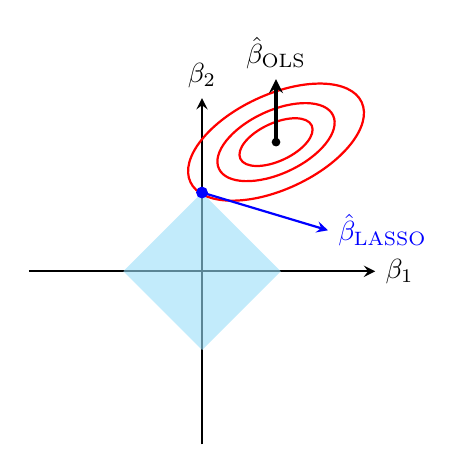
\begin{tikzpicture}[>=stealth, scale=2, thick]

  % Axes
  \draw[->] (-1.1,0) -- (1.1,0) node[right] {$\beta_1$};
  \draw[->] (0,-1.1) -- (0,1.1) node[above] {$\beta_2$};

  % LASSO constraint (diamond)
  \fill[cyan!40, opacity=0.6]
    (0,0.5) -- (0.5,0) -- (0,-0.5) -- (-0.5,0) -- cycle;

 % OLS ellipses
  \draw[red, thick, rotate around={25:(0.47,0.82)}] (0.47,0.82) ellipse (0.6 and 0.3);
  \draw[red, thick, rotate around={25:(0.47,0.82)}] (0.47,0.82) ellipse (0.4 and 0.2);
  \draw[red, thick, rotate around={25:(0.47,0.82)}] (0.47,0.82) ellipse (0.25 and 0.12);

  % Beta hat (OLS)
  \filldraw[black] (0.47, 0.82) circle (0.02);

  % Intersection point (LASSO)
  \filldraw[blue] (0,0.5) circle (0.03);
  \draw[->, blue, thick] (0,0.5) -- (0.8, 0.26);
  \node[blue, right] at (0.8, 0.26) {$\hat{\beta}_{\text{LASSO}}$};

  % Arrow to OLS
  \draw[->, very thick] (0.47,0.82) -- (0.47,1.22);
  \node[above] at (0.47,1.22) {$\hat{\beta}_{\text{OLS}}$};
\end{tikzpicture}
\caption{LASSO Optimization}
\label{fig:lasso_opt}
\end{figure}

As shown in Figure~\ref{fig:lasso_opt}, due to the optimization constraint and the design of penalization, LASSO performs variable selection and shrinks redundant or less impactful coefficients to 0. The tuning parameter $\lambda$ often determines the severity of penalization, the optimal value is obtained from cross validation. 

\subsection{Ridge}
Consider the linear regression model, but subject to penalization of model complexity
$$
y_t = \beta_0 + \beta_1 x_{1t} + \cdots + \beta_p x_{pt} + \epsilon_t, \quad t = 1, \hdots, T \text{ subject to } \sum_{j = 1}^p \beta_j^2 < \delta
$$
where $\delta$ is the threshold. Then, the \textbf{Ridge regression estimate} of a linear model is defined as 
$$
\hat{\boldsymbol\beta}^{\text{Ridge}} := \arg\min_{\boldsymbol\beta} \left\{ \sum_{t=1}^T \left(y_t - \beta_0 - \sum_{i=1}^p x_{it}\beta_i\right)^2 + \lambda \sum_{j=1}^p \beta_j^2\right\}
$$
where $\lambda > 0$ is a tuning parameter which determines the bias-variance trade-off and $\mathrm{Pen}$ function is $\ell_2$ norm (squared euclidean length of the parameters). Moreover, it has a closed form solution in matrix form 
$$
\textcolor{cyan}{\hat{\boldsymbol\beta}_{\text{Ridge}}} = \textcolor{cyan}{(\textbf{X}^T\textbf{X} + \lambda I_p)^{-1} \textbf{X}^T (\textbf{y} - \hat{\beta}_0 \textbf{1})}, \quad \textcolor{red}{\hat{\beta}_0} = \bar{y} - \frac{1}{n}\sum_{i=1}^n\sum_{j=1}^p \hat{\beta}_j x_{ij} = \textcolor{red}{ \bar{y} - \hat{\boldsymbol\beta}^T_{\text{Ridge}} \bar{\textbf{x}}}
$$

\begin{figure}[h]
\centering
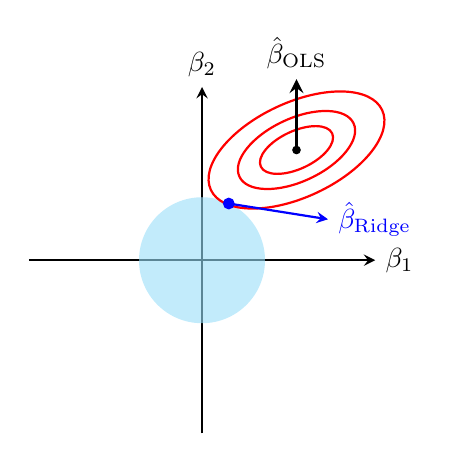
\begin{tikzpicture}[>=stealth, scale=2, thick]

  % Axes
  \draw[->] (-1.1,0) -- (1.1,0) node[right] {$\beta_1$};
  \draw[->] (0,-1.1) -- (0,1.1) node[above] {$\beta_2$};

  % Ridge constraint (circle)
  \fill[cyan!40, opacity=0.6] (0,0) circle (0.4);

  % OLS ellipses
  \draw[red, thick, rotate around={25:(0.6,0.7)}] (0.6,0.7) ellipse (0.6 and 0.3);
  \draw[red, thick, rotate around={25:(0.6,0.7)}] (0.6,0.7) ellipse (0.4 and 0.2);
  \draw[red, thick, rotate around={25:(0.6,0.7)}] (0.6,0.7) ellipse (0.25 and 0.12);

  % Beta hat (OLS)
  \filldraw[black] (0.6,0.7) circle (0.02);

  % Intersection point (Ridge)
  \filldraw[blue] (0.17,0.36) circle (0.03);
  \draw[->, blue, thick] (0.17,0.36) -- (0.8,0.26);
  \node[blue, right] at (0.8,0.26) {$\hat{\beta}_{\text{Ridge}}$};

  % Arrow to OLS
  \draw[->, very thick] (0.6,0.7) -- (0.6,1.15);
  \node[above] at (0.6,1.15) {$\hat{\beta}_{\text{OLS}}$};

\end{tikzpicture}
\caption{Ridge Optimization}
\label{fig:ridge_opt}
\end{figure}
As shown in Figure~\ref{fig:ridge_opt}, due to the optimization constraint and the design of penalization, Ridge does not perform variable selection directly like LASSO. The model shrinks some redundant or less impactful coefficients close to 0. The tuning parameter $\lambda$ often determines the severity of penalization, the optimal value is obtained from cross validation. 

\subsection{Random Forest}
A popular method in machine learning is the use of classification or decision trees. The algorithm is to split the large dataset into smaller and homogeneous groups based on their characteristics. The split aims to explain the variation in the response variable. Usually, the best split is determined to minimize a certain metric (such as Gini, Entropy and etc) that researchers choose. However, there are significant drawbacks to this approach, as single decision tree is prone to overfitting and the prediction changes drastically as the dataset changes. Moreover, there are also concerns with mis-classification, biases and inefficiencies when the number of predictors increases. \newline

To solve the issue, we consider one approach in ensemble learning, which is known as \textbf{bagging} (\textbf{B}ootstrap \textbf{Agg}regat\textbf{ing}). This is a classic algorithm, where multiple learning algorithms with different predictors are trained together, and the predictors are selected using bootstrap - a resampling method without replacement.

\begin{figure}[H]
\centering
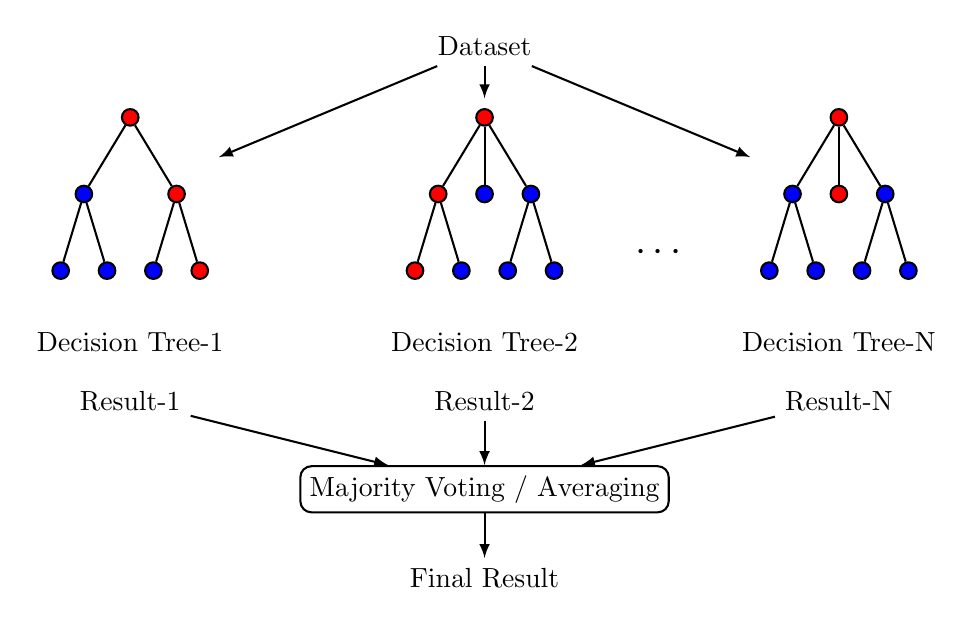
\begin{tikzpicture}[scale = 0.75]

% Top node
\node (data) at (0,1) {Dataset};

% -------- Tree 1 --------
\node (tree1) at (-6,-1.5) {
\begin{forest}
for tree={
    circle,
    draw,
    minimum size=6pt,
    inner sep=0pt,
    l sep=12pt,
    s sep=10pt
}
[ , fill=red
    [ , fill=blue
        [ , fill=blue]
        [ , fill=blue]
    ]
    [ , fill=red
        [ , fill=blue]
        [ , fill=red]
    ]
]
\end{forest}
};

\node at (-6,-4) {Decision Tree-1};
\node (r1) at (-6,-5) {Result-1};

% -------- Tree 2 --------
\node (tree2) at (0,-1.5) {
\begin{forest}
for tree={
    circle,
    draw,
    minimum size=6pt,
    inner sep=0pt,
    l sep=12pt,
    s sep=10pt
}
[ , fill=red
    [ , fill=red
        [ , fill=red]
        [ , fill=blue]
    ]
    [ , fill=blue]
    [ , fill=blue
        [ , fill=blue]
        [ , fill=blue]
    ]
]
\end{forest}
};

\node at (0,-4) {Decision Tree-2};
\node (r2) at (0,-5) {Result-2};

% -------- Tree N --------
\node (tree3) at (6,-1.5) {
\begin{forest}
for tree={
    circle,
    draw,
    minimum size=6pt,
    inner sep=0pt,
    l sep=12pt,
    s sep=10pt
}
[ , fill=red
    [ , fill=blue
        [ , fill=blue]
        [ , fill=blue]
    ]
    [ , fill=red]
    [ , fill=blue
        [ , fill=blue]
        [ , fill=blue]
    ]
]
\end{forest}
};

\node at (6,-4) {Decision Tree-N};
\node (r3) at (6,-5) {Result-N};

% Connections from dataset
\draw[->] (data) -- (tree1);
\draw[->] (data) -- (tree2);
\draw[->] (data) -- (tree3);

% Voting box
\node[draw, rectangle, rounded corners, minimum width=4cm] (vote) at (0,-6.5)
{Majority Voting / Averaging};

% Final result
\node (final) at (0,-8) {Final Result};

% Arrows
\draw[->] (r1) -- (vote);
\draw[->] (r2) -- (vote);
\draw[->] (r3) -- (vote);
\draw[->] (vote) -- (final);

% Dots between trees
\node at (3,-2.5) {\Large $\cdots$};

\end{tikzpicture}
\caption{Illustration of Random Forest (Bagging)}
\label{fig:rf}
\end{figure}

As shown in Figure~\ref{fig:rf}, each decision tree is built from random subset of the total predictors, and the resulting predictions for each tree are then aggregated using averaging or majority voting. The purpose of random selecting predictor ensures the diversity of the trees and largely reduce the risks of overfitting, moreover, the averaging or majority voting reduces the variance and ensures the robustness of the model.  \newline

In general, we tune the number of individual trees we want to have in the forest through cross validation, and typically more trees provide accurate predictions until a certain number. Other factors such as the depth/complexity of the tree, number of features to retain for a single tree and the subsamples sizes to learn could all be tuned based on validation. 

\subsection{Extreme Gradient Boosting (XGBoost)}
Another ensemble learning algorithm to consider is \textbf{boosting}. As opposed to random forest (bagging) where multiple learning algorithms are trained in parallel, this algorithm trains sequentially. In each steps of training, it creates new algorithm to make correction on errors of the previous trees. The final predictions are determined by the weighted combination of all learning algorithms, placing more emphasis by assigning larger weights on better performed algorithm. \newline

A boosted tree can be expressed as 
$$
\tilde{y}_i = m_J(x_i) = \sum_{j = 1}^J T_j(x_i)
$$
which represents the final prediction for $i^{\text{th}}$ data point, where it is simply a sum of the predictions from all $J$ trees in the model, where
$$
m_J(x_i) = \textcolor{blue}{\underbrace{m_{J - 1}(x_i)}_{\text{Old Trees}}} + \textcolor{red}{\underbrace{T_J(x_i)}_{\text{New Tree}}}
$$
and the new tree ($T_j$) is selected based on fitting the residuals of the previous model ($m_{J - 1}$). This process continues iteratively until the model's residual is minimized. \newline

The Extreme Gradient Boosting (XGBoost) algorithm uses boosting tree algorithm as foundation and minimizes the objective function $O$ defined as follows
$$
O = \underbrace{\sum_{i = 1}^n (y_i - \tilde{y}_i)^2}_{\text{Loss Function}} + \underbrace{\sum_{j = 1}^J \Omega(T_j)}_{\text{Penalty}}
$$
where the loss function is typically the squared error loss and the penalty is present to prevent building complex models. In other words, XGBoost aims to find prediction that balances both minimizations on the error and the complexity, which are typically trade-offs in predictive modelling. \newline

The penalization function is typically in the form 
$$
\Omega(T) = \gamma L + \frac{\lambda}{2} \sum_{i = 1}^L w_i^2
$$
where we penalize the number of leaves through $\gamma L$ and magnitude of output values through $\frac{\lambda}{2}\sum\limits_{i = 1}^L w_i^2$ ($w_i$ are specific prediction score to the $i^{\text{th}}$ leaf node). These tuning parameters $\lambda$ and $\gamma$, are typically obtained using validation. 

\subsection{Neural Network}
In finance, data are typically noisy or non-stationary, and this phenomenon complicates the process of separating the "signals" from the "noise" in the data. Therefore, neural network is often deployed to potentially isolate the "signals" to make accurate predictions.  


% NEURAL NETWORK with coefficients, shifted
\begin{figure}[h]
\centering
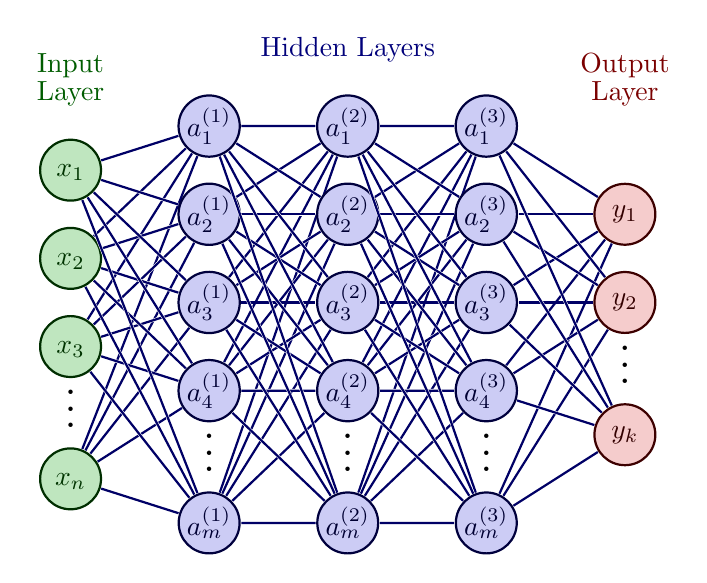
\begin{tikzpicture}[x=2.2cm,y=1.4cm, scale = 0.8]
  \message{^^JNeural network, shifted}
  \readlist\Nnod{4,5,5,5,3} % array of number of nodes per layer
  \readlist\Nstr{n,m,m,m,k} % array of string number of nodes per layer
  \readlist\Cstr{\strut x,a^{(\prev)},a^{(\prev)},a^{(\prev)},y} % array of coefficient symbol per layer
  \def\yshift{0.5} % shift last node for dots
  
  \message{^^J  Layer}
  \foreachitem \N \in \Nnod{ % loop over layers
    \def\lay{\Ncnt} % alias of index of current layer
    \pgfmathsetmacro\prev{int(\Ncnt-1)} % number of previous layer
    \message{\lay,}
    \foreach \i [evaluate={\c=int(\i==\N); \y=\N/2-\i-\c*\yshift;
                 \index=(\i<\N?int(\i):"\Nstr[\lay]");
                 \x=\lay; \n=\nstyle;}] in {1,...,\N}{ % loop over nodes
      % NODES
      \node[node \n] (N\lay-\i) at (\x,\y) {$\Cstr[\lay]_{\index}$};
      
      % CONNECTIONS
      \ifnum\lay>1 % connect to previous layer
        \foreach \j in {1,...,\Nnod[\prev]}{ % loop over nodes in previous layer
          \draw[connect,white,line width=1.2] (N\prev-\j) -- (N\lay-\i);
          \draw[connect] (N\prev-\j) -- (N\lay-\i);
          %\draw[connect] (N\prev-\j.0) -- (N\lay-\i.180); % connect to left
        }
      \fi % else: nothing to connect first layer
      
    }
    \path (N\lay-\N) --++ (0,1+\yshift) node[midway,scale=1.5] {$\vdots$};
  }
  
  % LABELS
  \node[above=0.2,align=center,mygreen!60!black] at (N1-1.90) {Input\\[-0.2em]Layer};
  \node[above=0.2,align=center,myblue!60!black] at (N3-1.90) {Hidden Layers};
  \node[above=0.6,align=center,myred!60!black] at (N\Nnodlen-1.90) {Output\\[-0.2em]Layer};
  
\end{tikzpicture}
\caption{Multilayer Perceptron Architecture}
\label{nn}
\end{figure}
The building block of neural network is the use of \textbf{perceptrons} - similar to a linear model to which is applied to a particular function, which is known as \textbf{activation functions}. The purpose of these functions is to introduce non-linearity to the linear models. As depicted in Figure~\ref{nn}, it is similar to the analogy of random forest, the input layer nodes (i.e., neurons) are fed to the perceptrons in the hidden layer (blue circles), where neural network combines them and each respective output is activated by the selected activation functions to produce the results. Hence, this model is also called \textbf{Multilayer Perceptron (MLP)} or \textbf{Feed Forward Neural Network (FNN)}. \newline

As mentioned earlier, activation function is crucial in multilayer perceptron, as it directly introduces non-linearity to the model. Common activation functions used are Tanh, ReLu, Softmax and etc. In general, the choice of activation function depends on the type of predictions, for example, ReLu is a popular choice for modelling option strategies, as the form is similar to an option payoff. \newline

Since the objective for neural network is minimizing the sum of least squares between the model and actual response variables, we have to be aware of the architecture where having too many layers may increase the risk of overfitting. Thus, it is possible to pose constraints and penalizations to reduce overfitting, consider the following objective function 
$$
O = \sum_{j = 1}^I \operatorname{loss}(y_i, \tilde{y}_i) + \sum_k \lambda k \lVert \textbf{W}_k \rVert_1 + \sum_j \lVert \textbf{W}_j \rVert_2^2
$$
where subscripts $k$ and $j$ represents the weights to which the $L_1$ and (or) $L_2$ penalization is applied. This function aims to directly limits the weights during the training. Another strategy is \textbf{dropout}, where the number of parameters of the model is reduced. 

\section{Related Work}
GPR 2 is an extension and application of the ideas proposed in GPR 1 with subtle modifications. All diagrams and explanations from Section 4 are inspired from the course materials presented in AFM/ACTSC 423 (Topics in Financial Econometrics) and STAT 443 (Forecasting). 

\newpage

\section{Experimental Methodology}
The dataset is collected from a researcher in Macroeconomics and Quantitative Finance - Philipp Dubach via GitHub (\textcolor{magenta}{\texttt{https://github.com/philippdubach/options-data}}), which holds a valid MIT license that permits distribution, modifications and so on. The dataset contains historical options data for 104 major US equities and ETFs, spanning from 2008 to 2025 with over 20 millions observations. For computational efficiency, we select the most recent data which is from 2024 to 2025. The data will be split into training data, testing data (for validation) and out of sample data:
\begin{itemize}
\item Training data spans from Jan 1st, 2024 to July 31st, 2024
\item Testing data spans from Aug 1st, 2024 to Sep 30th, 2024
\item Out of Sample data spans from Oct 1st, 2024 to Oct 31st, 2024
\end{itemize}
\subsection{Data Preprocessing}
Out of 104 major US equities, we select 10 for research purposes. These equities include Apple, Tesla, JPM, Amazon, NVIDA, Microsoft and so on. Then we apply filtration as entailed in GPR 1 to the data:
\begin{itemize}
\item Exclude options with no implied volatility and greeks 
\item Exclude options with zero volume over the last 7 calendar days
\item Remove options with bid price of 0
\end{itemize}
A verification on the bound of the option prices is also included to ensure the bound of American options are not violated. We remove any contracts from the data that violates this bound. After preliminary cleaning, the delta-hedged option rate of return is calculated using the formula in section 3.3, where realized delta, stock price and option price are obtained from the dataset. This return measures any excess return per day after accounting for hedge adjustments and financing costs. Note that delta-hedging is applied each trading day and for simplicity, we will not factor in transaction costs. \newline

To prevent potential data leakage and look-ahead bias, we mimic the real trading scenarios and roll the relevant predictors by one day, in other words, for each trading day, the information of these predictors are from yesterday. These predictors are selected based on whether we think the traders know these information at the beginning of the trading day. For example, an option's last traded price is typically known at the end of the trading day, so we definitely roll them to prevent leakage. Since the researcher did not explicitly mention the model they used to calculate option greeks, we choose to be conservative and also roll these variables by a day to limit look-ahead bias. Other variables such as time to maturity, moneyness and so on are evaluated to be available for model training. \newline

Then, we check the distribution of the predictors to determine the skewness and scale. Normalization is used on the training data and applied to the testing and out of sample data to prevent any leakage. To handle the outliers in response variable (i.e., the return), we realized that the return can simply explode if the denominator is too small. Since there is no actual economic meanings for huge returns, we choose to apply winsorization on the response to set a cap for the maximum and lowest return without deleting the outliers. This procedure is done carefully by selecting the 1\% quantile in the training data as lower bound and the 99.9\% quantile in the training data as upper bound. If any observations in the training data has return over (below) the upper (lower) bound, it will be capped off. These bounds are then applied to testing and out of sample data to prevent leakage. 

\subsection{Model Fitting}
After processing, we train the machine learning model Ridge, Lasso, Random Forest, XGBoost and Neural network using the training data. The tuning parameters are chosen via validation with some chosen arbitrarily based on the features. Then, measures such as mean squared error (MSE) and hit ratio are calculated based on the model's performance in testing data. Below are R packages we used for each model:
\begin{itemize}
\item Ridge: \texttt{glmnet}
\item Lasso: \texttt{glmnet}
\item Random Forest: \texttt{randomForest}
\item XGBoost: \texttt{xgboost}
\item Neural Network: \texttt{keras} and \texttt{tensorflow}
\end{itemize}
Note for better operations of Keras and Tensorflow, it is recommended to install Python 3.10, as newer versions have conflicts with the use of these packages. 

\subsection{Portfolio Construction}
For evaluating portfolio performance, we use the out-of-sample data and group all the contracts each day into deciles and construct three types of portfolios:
\begin{enumerate}
\item Long-Short Portfolio: Long decile 10 (highest predicted returns) and short decile 1 (lowest predicted returns)
\item Long-Only Portfolio: Long decile 10 (highest predicted returns)
\item Short-Only Portfolio: Short decile 1 (lowest predicted returns)
\end{enumerate}
We record the return for each day and compare between each models. Note that the rankings are determined by the predicted returns of each machine learning models. A lag of one day is introduced in the predicted return to prevent look ahead bias and mimic real trading. For computational simplicity, transaction costs for each portfolios are excluded and equal weighting is applied within each deciles. We are also aware that there are 252 trading days in a year, thus when calculating Sharpe ratio, the scale of 252 days is used rather than 365 days.  \newline

All the diagrams are generated either using R's embedded plot functions or \texttt{ggplot2}. For additional analysis, we also used \texttt{PerformanceAnalytics} to calculate measures such as max drawdown and so on. 

\newpage

\section{Results and Discussion}
This section will be divided into couple subsections that describes each model's predictive performance on the training, testing and out-of-sample data, profitability of constructed portfolio based on predictions and the analysis on the market to explain the profits. 

\subsection{Model Description and Performance}
For some machine learning algorithms, especially tree-based, the model typically learns the specific pattern in the training data very quickly, which usually leads to overfitting. With this in mind, we have indicated learning rate and penalization terms in our model to potentially limit overfitting. 

\begin{table}[h!]
\centering
\begin{tabular}{p{3cm} p{11cm}}
\toprule
\textbf{Model} & \textbf{Description} \\
\midrule

Ridge & Tuning parameter $\lambda$ selected via cross-validation. \\

& \\

Lasso & Tuning parameter $\lambda$ selected via cross-validation. \\

& \\

Random Forest & 
Sample size = 30{,}000; 
Node size = 250; 
Number of trees = 40; 
Number of predictors per split = 5. \\
& \\

XGBoost & 
Learning rate ($\eta$) = 0.3; 
Objective = squared error loss; 
Maximum depth = 4; 
$\lambda$ (L2 regularization) = 1; 
$\gamma$ (minimum loss reduction) = 0.1; 
Number of trees = 30. \\

& \\

Neural Network & 
Layer 1: ReLU, 16 units, input dimension = 26, L2 = 0.001; 
Dropout = 0.2; 
Layer 2: ReLU, 8 units, L2 = 0.001; 
Dropout = 0.2; 
Output layer: 1 unit. \\

\bottomrule
\end{tabular}
\caption{Model specifications and hyperparameters}
\end{table}
Note that most of the parameters are arbitrarily chosen based on our constraint and desired model complexity, however, parameters such as number of trees are decided based on the model's predictive performance on the testing data. 


\begin{table}[h!]
  \centering
  \begin{tabular}{cccccc}
  \hline
  & Ridge & Lasso & RF & XGBoost & NN \\
  \hline
\rule{0pt}{3ex} MSE & 0.0005269105 & \textbf{0.0005252877} & 0.0005310217 & 0.0005357839 & 0.0005292006 \\
 Hit Ratio & 0.5138297 & 0.5193873 & 0.4982097 & \textbf{0.5278039} & 0.4522442 \\
 \hline
 \end{tabular}
  \caption{Model Performance on Test Data}
  \label{perf_summary}
\end{table}

By inspection, most of the models in Table~\ref{perf_summary} have similar mean squared error. Noticeably, the machine learning models on average have slightly higher mean squared error than the linear models (such as Ridge and Lasso). This outcome is reasonable, since option data are often noisy, models such as Lasso and Ridge choose to ignore these noises by putting lower weights in the features that we selected (as depicted in Figure~\ref{heat}), therefore their results are generally biased. On the other hand, machine learning models utilize these features by studying the signals behind the noise, but the drawback is the increase in variance, hence yielding a relatively higher MSE. 

\begin{figure}[h]
\centering
\includegraphics[width=0.8\textwidth]{heat_map.pdf}
\caption{The weights on each features for all models (Out of Sample)}
\label{heat}
\end{figure}

In out of sample predictions, we can see that Lasso and Ridge all have coefficients extremely close to zero, their prediction is solely based on the intercept/bias term. Tree-based model places significant emphasis on stock characteristics such as the trading volume, open price and the highest price of the stock. Despite this phenomenon, all machine learning models have decent amount of weights on option-related characteristics, specifically, the bid-ask spread. This is consistent with other related work, since bid-ask spread is directly related to the liquidity of the option prices. Wider spread is a sign for low liquidity, high volatility and a high likelihood of pricing error. Narrower spread is a sign for high liquidity and efficient pricing. Therefore, it has high influence on hedged option return that is dependent on the volatility risk premium. Moreover, most of our machine learning model also consider the weights on option greeks, which are a key features to determine model mis-specifications and hedge errors. \newline

Another interesting discovery is that the hit ratios of the machine learning models are generally lower than linear-based models on average. This is also mainly due to linear-based models being conservative by shrinking all the parameters relating to each features close to zero. Thus, providing a smoother results than the machine learning models that are adapted to the noisy features. \newline

Hit ratios and mean squared error are generally crude measures as they treat all the predictions including extreme cases with same weight, therefore, we will discuss the ranking power of these models in the next section, which is directly related to portfolio construction.

\subsection{Portfolio Performance}
For portfolio construction, as we mentioned in section 6, three types of portfolios are constructed - long-short, long only and short only to examine the ranking power of all the models. Note that long-short portfolio is a more realistic trading strategy, whereas long only and short only are selected only to observe the model's selection on both ends.  

\subsubsection{Long-Short Portfolios}
\begin{table}[h!]
  \centering
  \begin{tabular}{cccccc}
  \hline
  & Ridge & Lasso & RF & XGBoost & NN \\
  \hline
\rule{0pt}{3ex} Portfolio Mean & -1.483e-04 & -7.305e-05 & 2.725e-05 & 3.013e-04 & \textbf{8.247e-04} \\
 Sharpe Ratio & -2.085106 & -2.693519 & -0.682621 &  0.864267 & \textbf{1.421018}  \\
 Max Drawdown & -1.0053 \% & -0.5921202 \% & -1.807707 \% & \textbf{-0.4757644 \%} & -2.381102 \% \\
 \hline
 \end{tabular}
  \caption{Long-Short Portfolio Performance for October 1, 2024 to November 1, 2024}
  \label{ls_port}
\end{table}

From Table~\ref{ls_port}, linear-based models perform worse on average than nonlinear models. The negative returns indicate that both Lasso and Ridge fail to rank the contracts on both ends, resulting the portfolio return to be significantly lower than the risk-free rate and leads to a negative sharpe ratio.\

\begin{figure}[h]
\centering
\includegraphics[width=0.76\textwidth]{long_short.pdf}
\caption{Daily performances of each model (Long Short)}
\label{ls_day}
\end{figure}

On the other hand, machine learning models such as XGBoost and Neural network provides positive profits on average and has a higher Sharpe Ratio, which also suggests that nonlinear models are possibly extracting useful economic signals from the data.  Although Neural Network yields the largest mean and sharpe ratio, but the max drawdown is also high, which suggests that the portfolio constructed is very volatile compared to other machine learning models. In contrast, XGBoost provides consistent portfolio within the month and have the least max drawdowns, which is a better choice for risk management relative to other models. \newline


From Figure~\ref{ls_day}, we can see that most non linear models perform better than linear-based models everyday. For Neural Network, the portfolio returns are extremely volatile with some performances extremely better or worse than others, which is consistent with the interpretation of Table~\ref{ls_port}.

\subsubsection{Long-Only Portfolios} 
\begin{table}[h!]
  \centering
  \begin{tabular}{cccccc}
  \hline
  & Ridge & Lasso & RF & XGBoost & NN \\
  \hline
\rule{0pt}{3ex} Portfolio Mean & -4.560e-04 & -4.041e-04 & -1.579e-04  & -1.949e-04 & \textbf{-5.085e-05} \\
 Sharpe Ratio & -2.3336402  & -2.0040015 & -1.2419322 & -1.2853664 & \textbf{-0.4987878} \\
 Max Drawdown &  -1.597888 \% & -1.679594 \% & \textbf{-0.9725774 \%} & -1.210067 \% & -3.029782 \% \\
 \hline
 \end{tabular}
  \caption{Long-Only Portfolio Performance for October 1, 2024 to November 1, 2024}
  \label{l_port}
\end{table}

Similar to long-short portfolio case, the nonlinear machine learning models outperform the linear-based models in ranking the contracts on average. Interestingly, all models yield negative returns in their portfolios, which shows they have poor performance in longing the "undervalued" contracts, in other words, the asset return did not grow as the model predicted. \newline


\begin{figure}[h]
\centering
\includegraphics[width=0.73\textwidth]{long_only.pdf}
\caption{Daily performances of each model (Long Only)}
\label{l_day}
\end{figure}

As shown in Table~\ref{l_port}, Neural Network provides the largest return compared to other models. However, the maximum drawdown for neural network reveals volatility and unstableness in the return. On the other hand, tree-based algorithms such as Random Forest and XGBoost all provide relatively stable results, despite having lower return than Neural Network. Lastly, both Lasso and Ridge performs worse with more volatile portfolio returns than other models. \newline

In Figure~\ref{l_day}, we observe similar results where non-linear models have higher return than linear-based models in most of the days. Noticeably, Neural Network have a huge spike for one day similar to the long-short portfolio case, where it significantly outperforms all other models. But, its returns are too volatile compared to other models that are relatively stable. 

\subsubsection{Short-Only Portfolios}
\begin{table}[h!]
  \centering
  \begin{tabular}{cccccc}
  \hline
  & Ridge & Lasso & RF & XGBoost & NN \\
  \hline
\rule{0pt}{3ex} Portfolio Mean & 0.0003076 & 0.0003310 & 0.0001851 & 0.0004963 & \textbf{0.0008755} \\
 Sharpe Ratio &  0.31658514 & 0.42505752 & -0.04170507 & 1.13241186  & \textbf{2.73623713} \\
 Max Drawdown &  -2.35283 \% & -2.185223 \% & -2.859081 \% & -1.626596 \% & \textbf{-1.062198 \%} \\
 \hline
 \end{tabular}
  \caption{Short-Only Portfolio Performance for October 1, 2024 to November 1, 2024}
  \label{s_port}
\end{table}

In contrast to long-only portfolios, all models have produced positive returns for the short-only portfolios, which reveals that the models are excellent at identifying the overvalued assets. Moreover, Neural Network excels not only in the mean return, but also provides a relatively stable portfolio with high Sharpe Ratio and low max drawdowns. On the other hand, as shown in Table~\ref{s_port}, the linear-based models are underperforming on average comparing to non-linear models except Random Forest. 

\begin{figure}[h]
\centering
\includegraphics[width=0.71\textwidth]{short_only.pdf}
\caption{Daily performances of each model (Short Only)}
\label{s_day}
\end{figure}

As seen in Figure~\ref{s_day}, non-linear models are performing better than linear models for most days. Noticeably, Neural Network is able to provide accurate ranking of overvalued assets for most of the days, which includes the extreme cases when all model performs badly. However, Random Forest is able to provide accurate ranking for most of the time, but severely underperforms in extreme cases, which provides less stable results compared to other algorithms. 



\subsection{Remarks and Analysis}
In this subsection, we will provide a summary of the performance of all models and analyze the models' ability of capturing the signals from noisy data, moreover, we will consider whether there are external factors that influence the models to provide these results.
\begin{figure}[h]
\centering
\includegraphics[width=0.62\textwidth]{efficiency_frontier.pdf}
\caption{Efficiency Frontier for all Models (Long Short Portfolio)}
\label{eff_front}
\end{figure}

Based on Figure~\ref{eff_front}, we can see the results are consistent with related works, as the frontiers of non-linear machine learning models tend to be more top-left compared to linear-based models. Moreover, we see XGBoost and Neural Network tend to provide larger expected returns when the risk increases. Note that some efficient frontiers are relatively "shorter", this suggests that these models produce portfolios with very similar risk-return across different weights. Similar to other relevant studies, the linear models are below the non-linear models. This reveals that their predictions are relatively conservative, especially for Ridge and Lasso whose prediction is based on the bias term, thus the volatility is much smaller and the returns are lower. From this figure, we can also see that Neural Network and XGBoost are excellent at capturing the non-linear signals between the features, while Random Forest, Ridge and Lasso failed to exploit the interactions between the features.  \newline

In previous literatures, there is a consensus that the model's predictability and profitability comes from the volatility risk premium, or in other words, the difference between the market's expected volatility (implied volatility) and the actual market's volatility. \newline

\begin{table}[h!]
  \centering
  \begin{tabular}{ccccccc}
  \hline
  & 1st Quantile & Median & Mean & 3rd Quantile & Kurtosis & Skew \\
  \hline
\rule{0pt}{3ex} Return & -0.738\% & -0.116\% & -0.045\% & 0.4895\% & 21.687 & 2.523  \\
Implied Volatility & 0.32707 & 0.50267 & 0.49750 & 0.57096 & 109.0016 & 6.722899 \\
Market Volatility & 0.2155 & 0.2566 & 0.3406  & 0.3676 & 0.5307571 & 1.357562 \\
Delta & -0.10179 & 0.06342  & 0.18866  & 0.63038 & -0.6931139 & -0.08344831 \\
Gamma & 0.00189 & 0.00424 & 0.00763 & 0.00861 & 9644.31 & 71.0384 \\
 \hline
 \end{tabular}
  \caption{Out of Sample Data Summary (Oct 1, 2024 to Nov 1, 2024)}
  \label{sum_out}
\end{table}

From the summary statistics presented in Table~\ref{sum_out}, we observed that the implied volatility is on average higher than the market's actual volatility (the average of mean volatility for each stocks), which means overestimation to the market's future volatility and the option prices embed compensations for bearing volatility risk. Thus, creating opportunities to isolate risk premiums, which is a key factor in delta-hedged option returns. Moreover, the return distribution has a slightly negative mean for the month, with strong positive skewness and excess kurtosis, this indicates that large positive outcomes can occur even when the mean is negative. This also explains why some of the model provides negative sharpe ratio and returns. \newline

In many option pricing models, implied volatility is a crucial input to calculate option greeks, such as Delta, Gamma and so on. For example, the formula to calculate delta in Black-Scholes model requires implied volatility to calculate delta, which estimates the probability of option expiring in-the-money in Black Scholes framework. However, since the implied volatility is higher than realized volatility, the resulting delta estimate may be biased. \newline

The discrepancies in the deltas can lead to hedging errors in delta-hedged portfolios, thus affecting our returns. To examine this, we will run diagnostic on the hedge errors on out of sample data to indicate the presence of systematic bias. Note that we are unable to include all hedge error plots of every contracts, we will extract one contract from out of sample data with obvious pattern for illustration. 

\begin{figure}[h]
\centering
\includegraphics[width=0.67\textwidth]{hedge_error.pdf}
\caption{Residual Analysis on Contract \texttt{AAPL250620C00330000}}
\label{hedge}
\end{figure}

In Figure~\ref{hedge}, we see that the hedge errors shows a strong negative linear relationship with the stock price change. Additionally, to test the statistical significance we fit a simple linear regression model using hedge error as response variate and stock price change as predictor. 

\begin{table}[h!]
  \centering
  \begin{tabular}{|ccccc|}
  \hline
  & Estimate & Std. Error & $t$ Value & Pr$(> |t|)$ \\
  \hline
\rule{0pt}{3ex} \texttt{(Intercept)} & -0.003521 & 0.010642  & -0.331  & 0.744 \\
\texttt{dS}          & -0.021991  &  0.003854 &  -5.706  & 1.39e-05 *** \\
 \hline
 \end{tabular}
  \caption{Output of Simple Linear Regression for Residual Analysis}
  \label{lin_reg}
\end{table}

This is a very informative result, as the slope coefficient is indeed statistically significant. This shows the deltas in our data are systematically biased and the option pricing model is over-hedging. In other words, the Delta-hedged return in our data does not fully cancel the directional impact of the stock. In our case, the models will most likely gain profit when the stock moves downward. This ties back to section 6.1, where we discovered most of our non linear models put more weights on stock-based features rather than option-based features.  Due to systematic bias, these non linear models prioritize the biased signal that is related to stocks rather than interpreting option-related features that embed signals for volatility risk premiums. In our case, those are relatively hard to capture since signals from the stocks are much stronger. Moreover, this is also the reason why all of our model yield positive returns with short-only portfolio, since Delta did not cancel out the directional impact of the stock, short position will provide profit and long position is often negative as shown in section 6.2.2 and 6.2.3. \newline

Having the bias in the delta in mind, an important remark is that the outperformance of nonlinear model appears to be influenced by the market conditions and bias in hedging. The generalization of these results on other market conditions are highly questionable, especially when the stock price movements move upwards or remain stable within the month. There are chances where the advantages of non linear machine model diminish and linear based model such as Lasso or Ridge outperforms. 


\section{Conclusion}
In conclusion, from our experiment, we observed the ability of non linear machine learning model at signal capturing is better comparing to linear based model. Moreover, we see that biased delta influence the learning of each model by focusing more on stock-based characteristics over option-based characteristics. However, there are several limitations. First, we were unable to obtain the option pricing model used that calculate the greeks and implied volatility, this increases the difficulty of investigating why deltas are systematically biased. Second, due to our limited access to the informations, we weren't able to gather more predictor variables for both options and stocks like the literatures reviewed in GPR 1, thus resulting in less information for the models to learn from. Future studies should continue investigating on the generalizability of this experiment onto different market conditions, and determine whether non linear models are still superior at capturing the stock-based signals compared to linear-based models when delta is biased. 

\newpage

\begin{center}
\textbf{Work Cited}
\end{center}
Black, F. \& Scholes. M. (1973). Pricing of Options and Corporate Liabilities. \textit{Journal of Political Economy}, 81(3), 637-654. \newline

Tian, M., and L. Wu. 2023. "Limits of Arbitrage and Primary Risk-Taking in Derivative Securities". \textit{The Review of Asset Pricing Studies} 13: 405-439. \newline

Ho, Steven Wei and Hu, Yutong. \textit{Option Return Predictability, A Machine-Learning Approach} (November 17, 2017). Available at SSRN: \textcolor{magenta}{\texttt{https://ssrn.com/abstract=3073791}} or \newline \textcolor{magenta}{\texttt{http://dx.doi.org/10.2139/ssrn.3073791}}. \newline

Huang, Y., Wang, Z. \& Xiao, Z. (2025). Option Return Predictability via Machine Learning: New Evidence From China. \textit{Journal of Futures Markets}, 45(9), 1232-1252. \newline \textcolor{magenta}{\texttt{https://doi.org/10.1002/fut.22604}}. \newline

Bali, T. G., Beckmeyer, H., Moerke, M., \& Weigert, F. (2023). Option Return Predictability with Machine Learning and Big Data. \textit{Review of Financial Studies}, 36(9), 3548–3602.


\end{document}